% !TeX TS-program = pdflatex
% !TeX encoding = UTF-8
% !TeX spellcheck = ru_RU-Russian
\documentclass{bmstu}
% !TeX TS-program = pdflatex
% !TeX encoding = UTF-8
% !TeX TXS-program:bibliography = biber
% !TeX spellcheck = ru_RU-Russian
\usepackage{pdfpages}
\usepackage{amsthm}
\PassOptionsToPackage{urldate=long}{biblatex}
% следующие 3 строчки нужны для точечек в содержании
\usepackage{tocloft}
\renewcommand{\cftpartleader}{\cftdotfill{\cftdotsep}}
\renewcommand{\cftchapleader}{\cftdotfill{\cftdotsep}}

% шапка в титульнике чтоб лучше стала
\renewcommand{\titlepageheader}[2]
{
	\begin{wrapfigure}[7]{l}{0.14\linewidth}
		\vspace{3.4mm}
		\hspace{-8mm}
		\includegraphics[width=0.89\linewidth]{bmstu-logo}
	\end{wrapfigure}
	
	{
		\singlespacing \small
		Министерство науки и высшего образования Российской Федерации \\
		Федеральное государственное бюджетное образовательное учреждение \\
		высшего образования \\
		<<Московский государственный технический университет \\
		имени Н.~Э.~Баумана \\
		(национальный исследовательский университет)>> \\
		(МГТУ им. Н.~Э.~Баумана) \\
	}
	
	\vspace{-4.2mm}
	\vhrulefill{0.9mm} \\
	\vspace{-7mm}
	\vhrulefill{0.2mm} \\
	\vspace{2.8mm}
	
	{
		\small
		ФАКУЛЬТЕТ \longunderline{<<#1>>} \\
		\vspace{3.3mm}
		КАФЕДРА \longunderline{#2} \\ % вот здесь убрал <<>>, чтобы
		% можно было подписать (ФН-11) вне кавычек 
	}
}
% Установка исполнителей работы
\renewcommand{\titlepageauthors}[5]
{
	{
		\renewcommand{\titlepagestudentscontent}{}
		\maketitlepagestudent{#1}
		
		\renewcommand{\titlepageotherscontent}{}
		\maketitlepageothers{#2}{#3}
		\maketitlepageothers{Консультант}{#4}
		\maketitlepageothers{Нормоконтролер}{#5}
		
		\small
		\begin{tabularx}{\textwidth}{@{}>{\hsize=.5\hsize}X>{\hsize=.25\hsize}X>{\hsize=.25\hsize}X@{}}
			\titlepagestudentscontent
			
			\titlepageotherscontent
		\end{tabularx}
	}
}


\renewcommand{\maketableofcontents}
{
	\setlength{\cftbeforetoctitleskip}{-2em}
	\setlength{\cftaftertoctitleskip}{0em}
	\renewcommand\contentsname{
	\normalsize \centerline{\MakeUppercase{Содержание}}\hfill c.
	}
%	\singlespacing
	\tableofcontents
}


\newif\ifgdeSep
\newcommand*{\gde}[1]{%
	\begin{enumerate}[itemindent=\parindent]
		\gdeSepfalse
		\item[где]
		\gdeScan#1\relax \text{.}
	\end{enumerate}
}
\newcommand{\gdeScan}[2]{%
	\ifx\relax#1\empty
	\else
	\ifgdeSep
	;\item[]\relax
	\else
	\gdeSeptrue
	\fi
	#1 -- #2\relax
	\expandafter\gdeScan
	\fi
}

\DeclareMathOperator{\Ch}{ch}
\DeclareMathOperator{\Sh}{sh}
\DeclareMathOperator{\Arctgh}{arctgh}

\DeclareMathOperator{\Arctg}{arctg}

\newenvironment{gost-itemize}
{\begin{itemize}[label=---,itemindent=\parindent,leftmargin=0pt]}
	{\end{itemize}}
	
\makeatletter
\newcommand{\oset}[3][0ex]{%
	\mathrel{\mathop{#3}\limits^{
			\vbox to#1{\kern-0\ex@
				\hbox{$\scriptstyle#2$}\vss}}}}
\makeatother
\newcommand*\protivorechie{$\oset{\circ}{\times}$}
%\newcommand*\protivorechie{$\times^{\kern-0.55em \circ}$}

\newcommand{\lineup}[5]{
	\newcommand*\lineupothercontent{}
	
	\newcommand{\makelineupother}[5]
	{
		\foreach \c in {#3} {
			\gappto\lineupothercontent{#2 &}
			\gappto\lineupothercontent{\fixunderline{}{40mm}{(Подпись, дата)} \vspace{1.3mm} &}
			\gappto\lineupothercontent{\fixunderline}
			\xappto\lineupothercontent{{\c}}
			\gappto\lineupothercontent{{40mm}{(И.~О.~Фамилия)} \\}
		}
		
		\foreach \s/\g in {#1} {
			\gappto\lineupothercontent{Исполнитель,\\студент группы \fixunderline}
			\xappto\lineupothercontent{{\g}}
			\gappto\lineupothercontent{{25mm}{(Группа)} &}
			\gappto\lineupothercontent{\fixunderline{}{40mm}{(Подпись, дата)} \vspace{1.3mm} &}
			\gappto\lineupothercontent{\fixunderline}
			\xappto\lineupothercontent{{\s}}
			\gappto\lineupothercontent{{40mm}{(И.~О.~Фамилия)} \\}
		}
		
		\foreach \c in {#5} {
			\gappto\lineupothercontent{#4 &}
			\gappto\lineupothercontent{\fixunderline{}{40mm}{(Подпись, дата)} \vspace{1.3mm} &}
			\gappto\lineupothercontent{\fixunderline}
			\xappto\lineupothercontent{{\c}}
			\gappto\lineupothercontent{{40mm}{(И.~О.~Фамилия)} \\}
		}
		
	}
	
	\makelineupother{#1}{#2}{#3}{#4}{#5}
	
	\centerline{\MakeUppercase{\textbf{Список исполнителей}}}
	
	\vspace{14mm}
	
	{\small\raggedright \begin{tabularx}{\textwidth}{@{}>{\hsize=.5\hsize}X>{\hsize=.25\hsize}X>{\hsize=.25\hsize}X@{}}
			\lineupothercontent
	\end{tabularx}}
	
	\pagebreak
}

\newcommand*{\QED}[1][$\square$]{%
	\leavevmode\unskip\penalty9999 \hbox{}\nobreak\hfill
	\quad\hbox{#1}%
}

\makeatletter
\newenvironment{sqcases}{%
	\matrix@check\sqcases\env@sqcases
}{%
	\endarray\right.%
}
\def\env@sqcases{%
	\let\@ifnextchar\new@ifnextchar
	\left\lbrack
	\def\arraystretch{1.2}%
	\array{@{}l@{\quad}l@{}}%
}
\makeatother

\def\doubleunderline#1{\underline{\underline{#1}}}

\newtheorem{opr}{Опредление}

\newcommand{\eqdef}{\overset{\mathrm{def}}{\equiv\joinrel\equiv}}
\usepackage{color}
\definecolor{lightgray}{rgb}{.9,.9,.9}
\definecolor{darkgray}{rgb}{.4,.4,.4}
\definecolor{purple}{rgb}{0.65, 0.12, 0.82}
\lstdefinelanguage{JavaScript}{
	keywords={break, case, catch, continue, debugger, default, delete, do, else, false, finally, for, function, if, in, instanceof, new, null, return, switch, this, throw, true, try, typeof, var, void, while, with},
	morecomment=[l]{//},
	morecomment=[s]{/*}{*/},
	morestring=[b]',
	morestring=[b]",
	ndkeywords={class, export, boolean, throw, implements, import, this},
	keywordstyle=\color{blue}\bfseries,
	ndkeywordstyle=\color{darkgray}\bfseries,
	identifierstyle=\color{black},
	commentstyle=\color{purple}\ttfamily,
	stringstyle=\color{red}\ttfamily,
	sensitive=true
}
\lstset{
	language=JavaScript,
	backgroundcolor=\color{lightgray},
	extendedchars=true,
	basicstyle=\footnotesize\ttfamily,
	showstringspaces=false,
	showspaces=false,
	numbers=left,
	numberstyle=\footnotesize,
	numbersep=9pt,
	tabsize=2,
	breaklines=true,
	showtabs=false,
	captionpos=b
}
\definecolor{numbers}{rgb}{0.5, 0.5, 0.5}
\definecolor{keywords}{rgb}{0.13, 0.13, 1}
\definecolor{comments}{rgb}{0, 0.5, 0}
\definecolor{strings}{rgb}{0.9, 0, 0}

% Команда создания листинга с подсветкой синтаксиса и нумерацией строк
\renewcommand{\includelistingpretty}[3]
{
	\lstinputlisting[
	language={#2},
	keywordstyle=\color{keywords},
	stringstyle=\color{strings},
	commentstyle=\color{comments},
	frame=leftline,
	numbers=left,
	numberstyle=\footnotesize\color{numbers},
	caption={#3},
	label={lst:#1},
	]{../src/#1}
}

\begin{document}
	\makereporttitle
	{Фундаментальные науки} % Название факультета
	{<<Вычислительная математика и математическая физика>> (ФН-11)} % Название кафедры
	{домашней работе №~1} % Название работы (в дат. падеже)
	{Компьютерная геометрия} % Название курса (необязательный аргумент)
	{} % Тема работы
	{} % Номер варианта (необязательный аргумент)
	{Куприн~А.~Д./ФН11-51Б} % Номер группы/ФИО студента (если авторов несколько, их необходимо разделить запятой)
	{Захаров~А.~А.} % ФИО преподавателя
	
	\maketableofcontents
	
	\chapter{Задание}
	Напишите программу, обеспечивающую воспроизведение движения планет вокруг Солнца в трёхмерном пространстве подобно
	той, что описана на стр. 135–138 книги [2]. Задайте угловую скорость вращения каждой планеты. Наклоните оси планет. Добавьте
	к паре планет их спутники (например, Луну для Земли и Фобос и
	Деймос для Марса).
	
	\chapter{Выполнение}
	Репозиторий: \url{https://github.com/Plasmaa0/webgl-solar-system}
	\begin{enumerate}
		\item Создал компонент \verb|WebGLCanvas| содержаший основной цикл выполнения программы. В нем задаются параметры камеры, создаются планеты, создается \verb|GUI|.
		
		\item Для реализации функционала камеры создан отдельный файл \verb*|Camera.js|, в котором написаны функции для получаения \verb*|view| и \verb*|projection| матриц. А также реализовано получения базиса камеры, а именно трех векторов направленных вперед по взгляду, направо и вверх. Это нужно для более приятного управления камерой на клавиши \verb*|W,A,S,D,Q,E| и стрелки.
		
		\item В файле \verb|Planet.js| создан класс планеты содержащий информацию о планете, параметрах ее орбиты, а также ее спутниках. Основные функции этого класса это:
		\begin{enumerate}
			\item \verb|update(deltaTime)| - обновляет положение планеты в пространстве, положение планеты потом используется для создания её \verb|model| матрицы. Реализация предельно простая, вытекает из школьной тригонометрии. Эта функция рекурсивно вызывается на всех спутниках планеты, которые сами по себе тоже являются представителями класса \verb|Planet|. Такая реализация позволяет за один вызов \verb|update()| на Солнце отрисовать рекурсивно сразу всю солнечную систему.
			\item \verb|draw(gl, shaderProgram, camera, params)| - аналогично \verb|update()| вызывается рекурсивно на всех спутниках. Такая реализация позволяет за один вызов \verb|draw()| на Солнце отрисовать рекурсивно сразу всю солнечную систему. Внутри функции в программе загружается нужный шейдер (для Солнца или остальных планет шейдеры отличаются из-за реализации света). После этого с помощью вспомогательных функций и методов получаются \verb|MVP| матрицы и загружаются в шейдер. Генерируются вершины изосферы с помощью \verb|generateSphereVertices()|. Они также используются в качестве нормалей, так как на единичной изосфере координаты её вершин равны нормалям этих вершин. Обзор шейдеров будет отдельным пунктом.
			\item \verb|generateSphereVertices()| - генерирует вершины изосферы с заданным количеством параллелей и меридианов.
		\end{enumerate}
		
		\item В файле \verb|shaders.js| находятся шейдеры для Солнца и остальных планет. Шейдер для солнца тривиален и рассмотрен не будет. Шейдер для планет является более продвинутым, так как в нем рассчитывается свет. В шейдер в момент вызова функции \verb|draw()| у планеты передается множество нужных параметров позволяющих реализовать освещение. Например, положение источника света, направление света, нормали поверхностей и так далее. Реализованы несколько алгоритмов освещения:
		\begin{enumerate}
			\item Глобальное освещение (направление одинаково везде). 
			\item Точечный (\verb|point|) источник света - применяется для симуляции света Солнца, в данный момент выключено. 
			\item\verb|Spot|-свет освещающий только узкий конус пространства, раствор которого можно контролировать через графический интерфейс.
			\item\verb|Ambient| - фоновое освещение - небольшая подсветка всех поверхностей независимо от того, попадает ли на них свет, или они находятся в темноте.
		\end{enumerate}
		Детали реализации взяты из лекций и сайта \url{webglfundamentals.org/webgl/lessons}.
		
	\end{enumerate}
	
	\begin{figure}
		\centering
		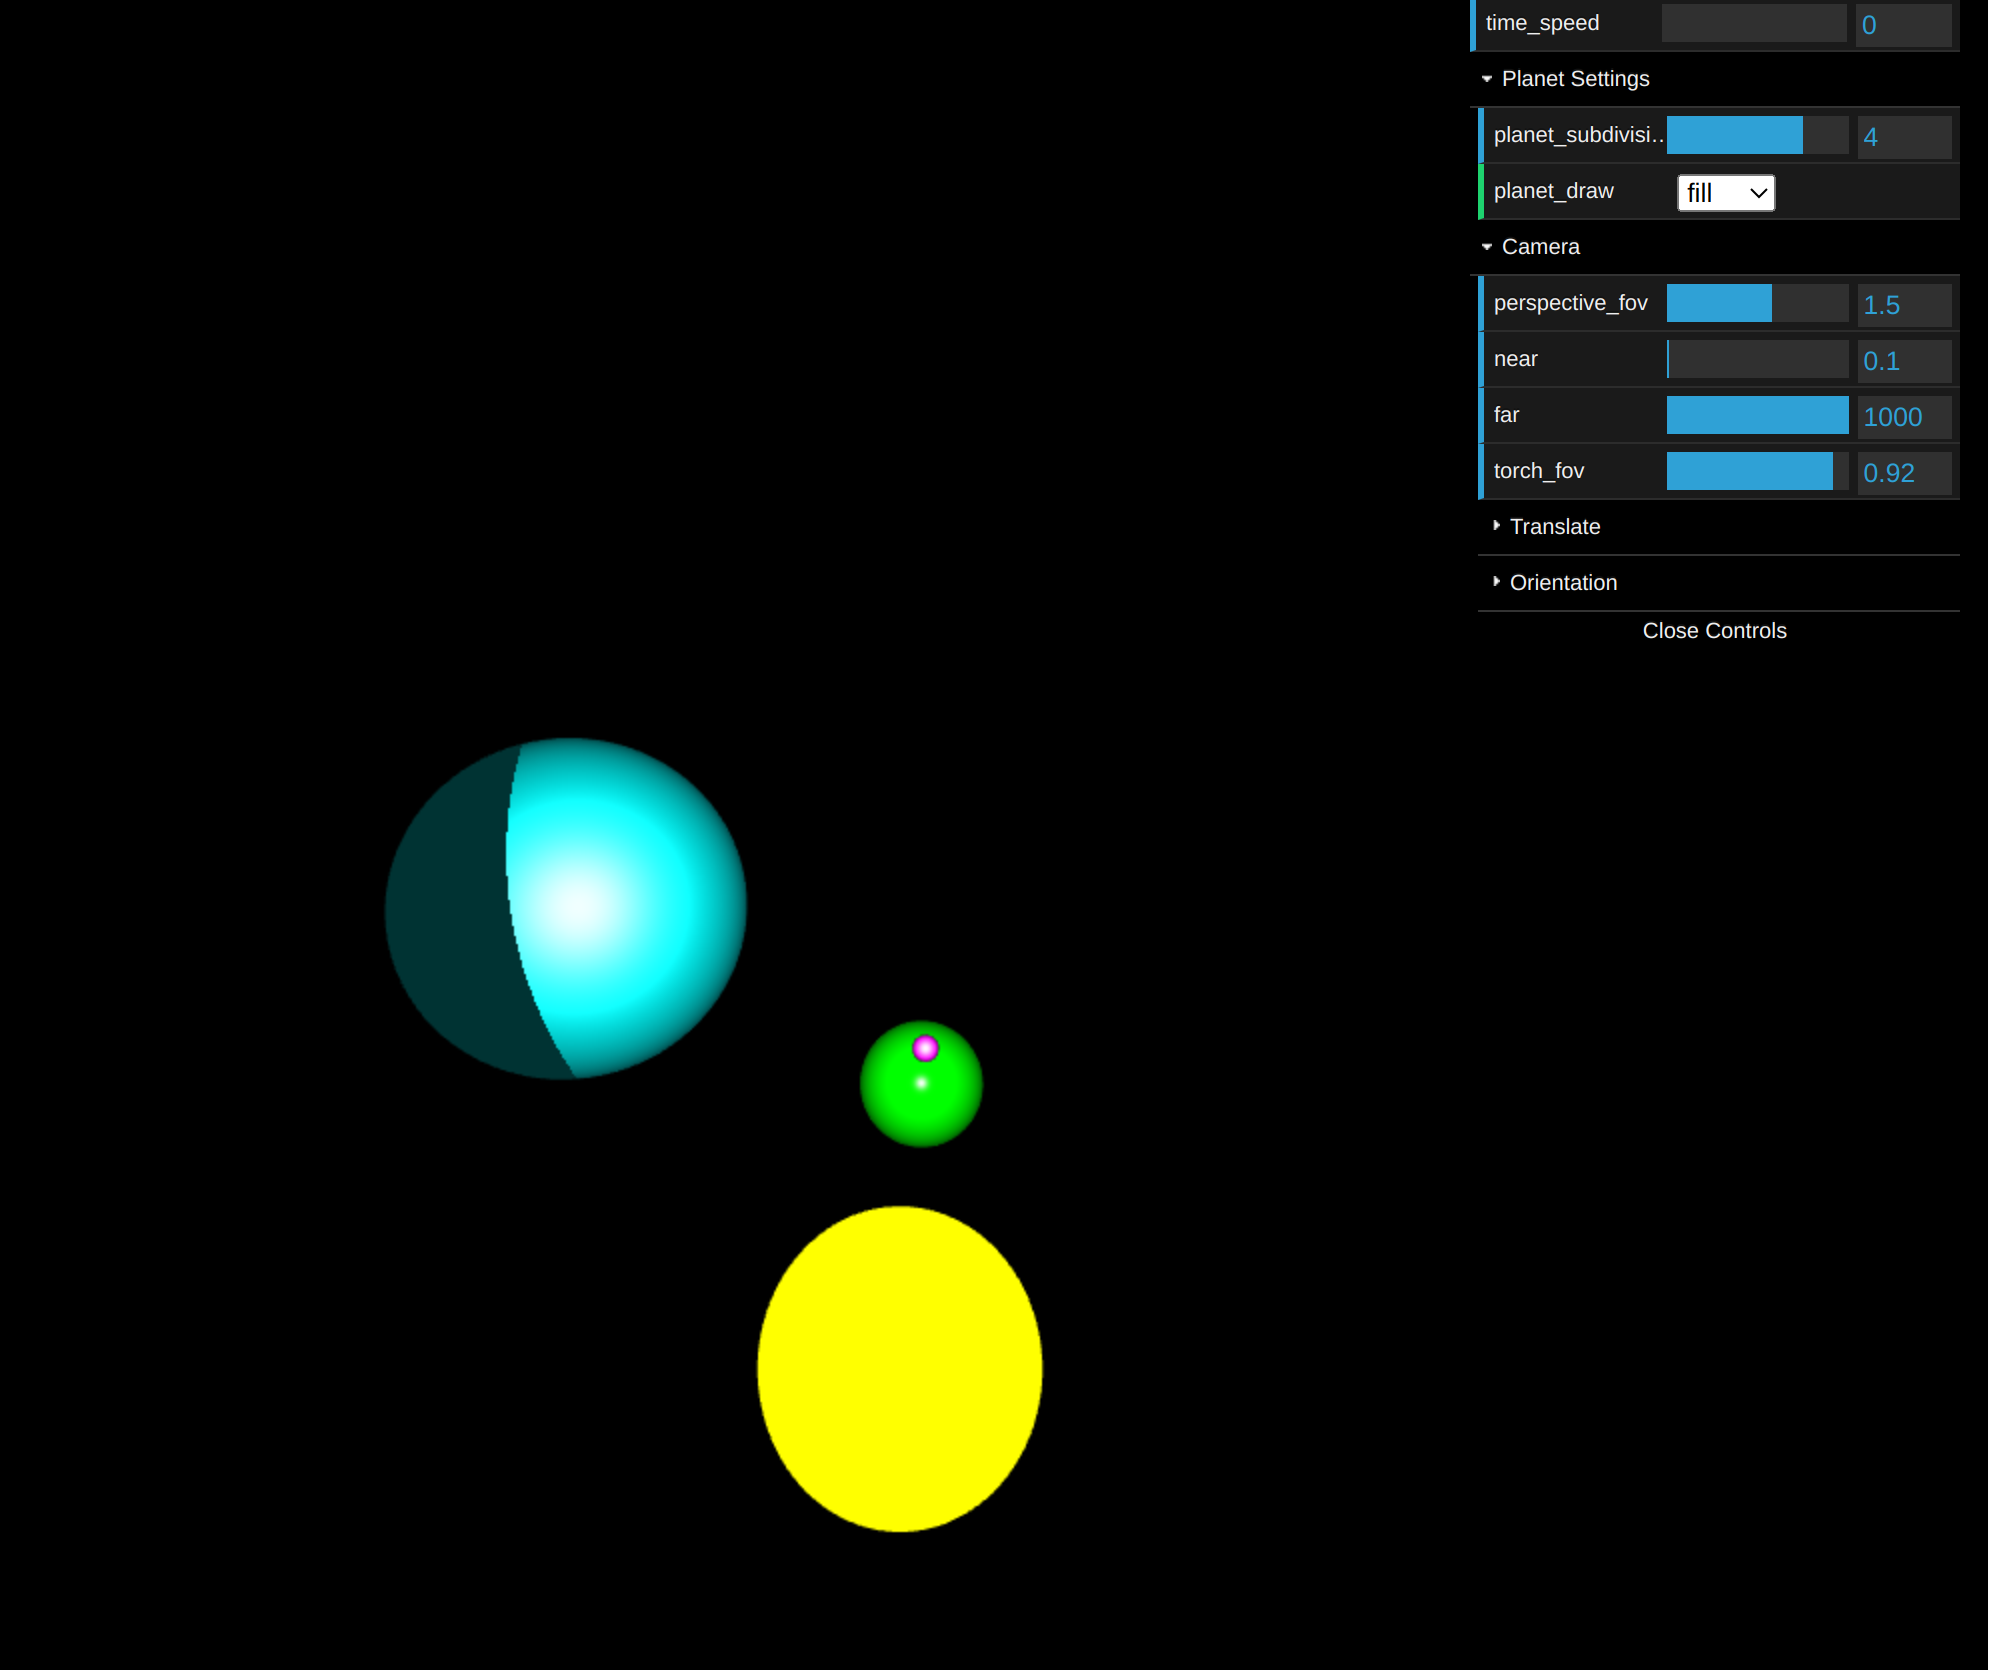
\includegraphics[width=\linewidth]{screenshot001}
		\caption{Пример системы из двух планет, у одной из которых есть спутник. Освещение - spotlight с небольшим раствором направленный из камеры вперед.}
		\label{fig:screenshot001}
	\end{figure}
	
	% TODO: \usepackage{graphicx} required
	\begin{figure}
		\centering
		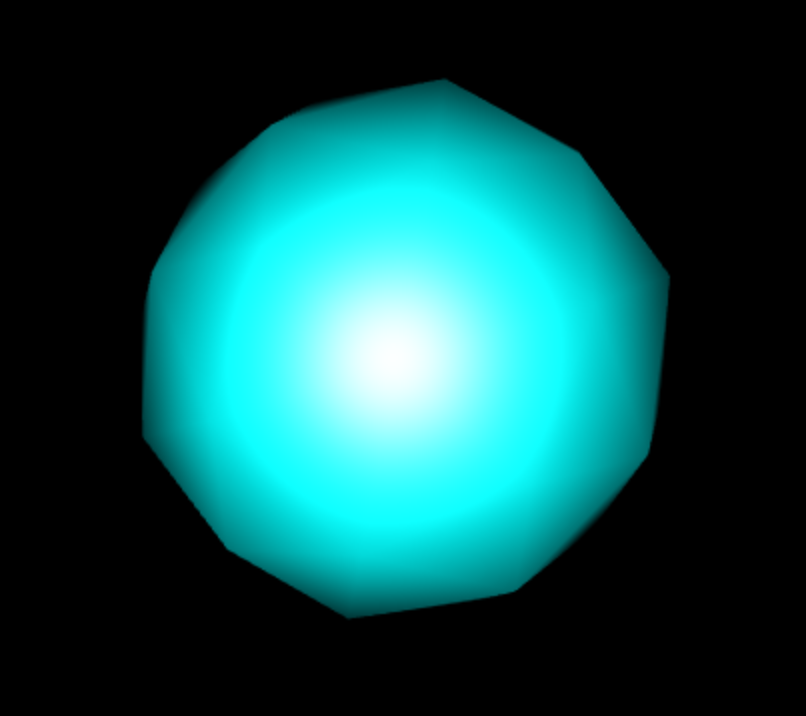
\includegraphics[width=0.4\linewidth]{lowres_planet}
		\centering
		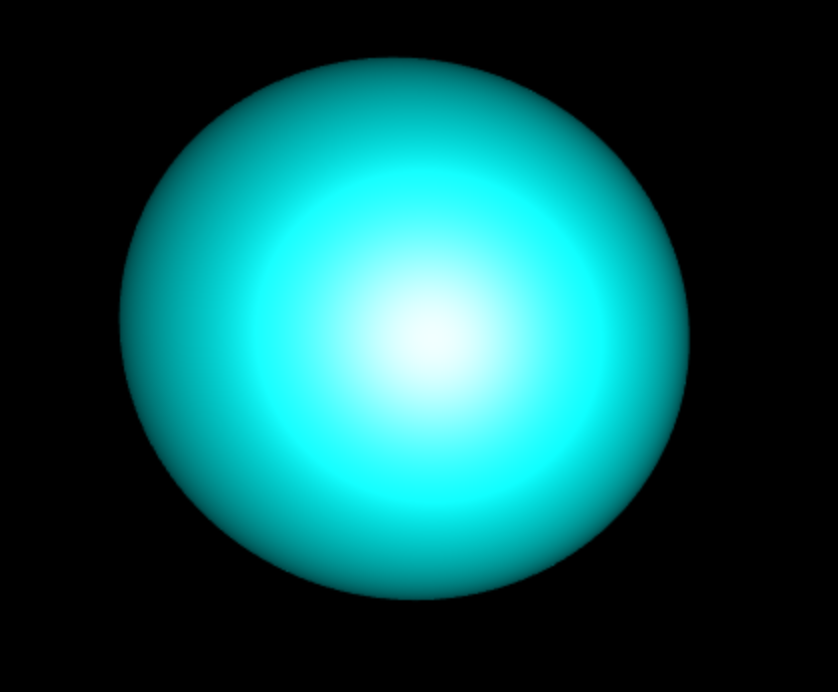
\includegraphics[width=0.4\linewidth]{highres_planet}
		\caption{Пример генерации изосферы с малым (слева) и большим (справа) количеством вершин.}
	\end{figure}
	
	% TODO: \usepackage{graphicx} required
	\begin{figure}
		\centering
		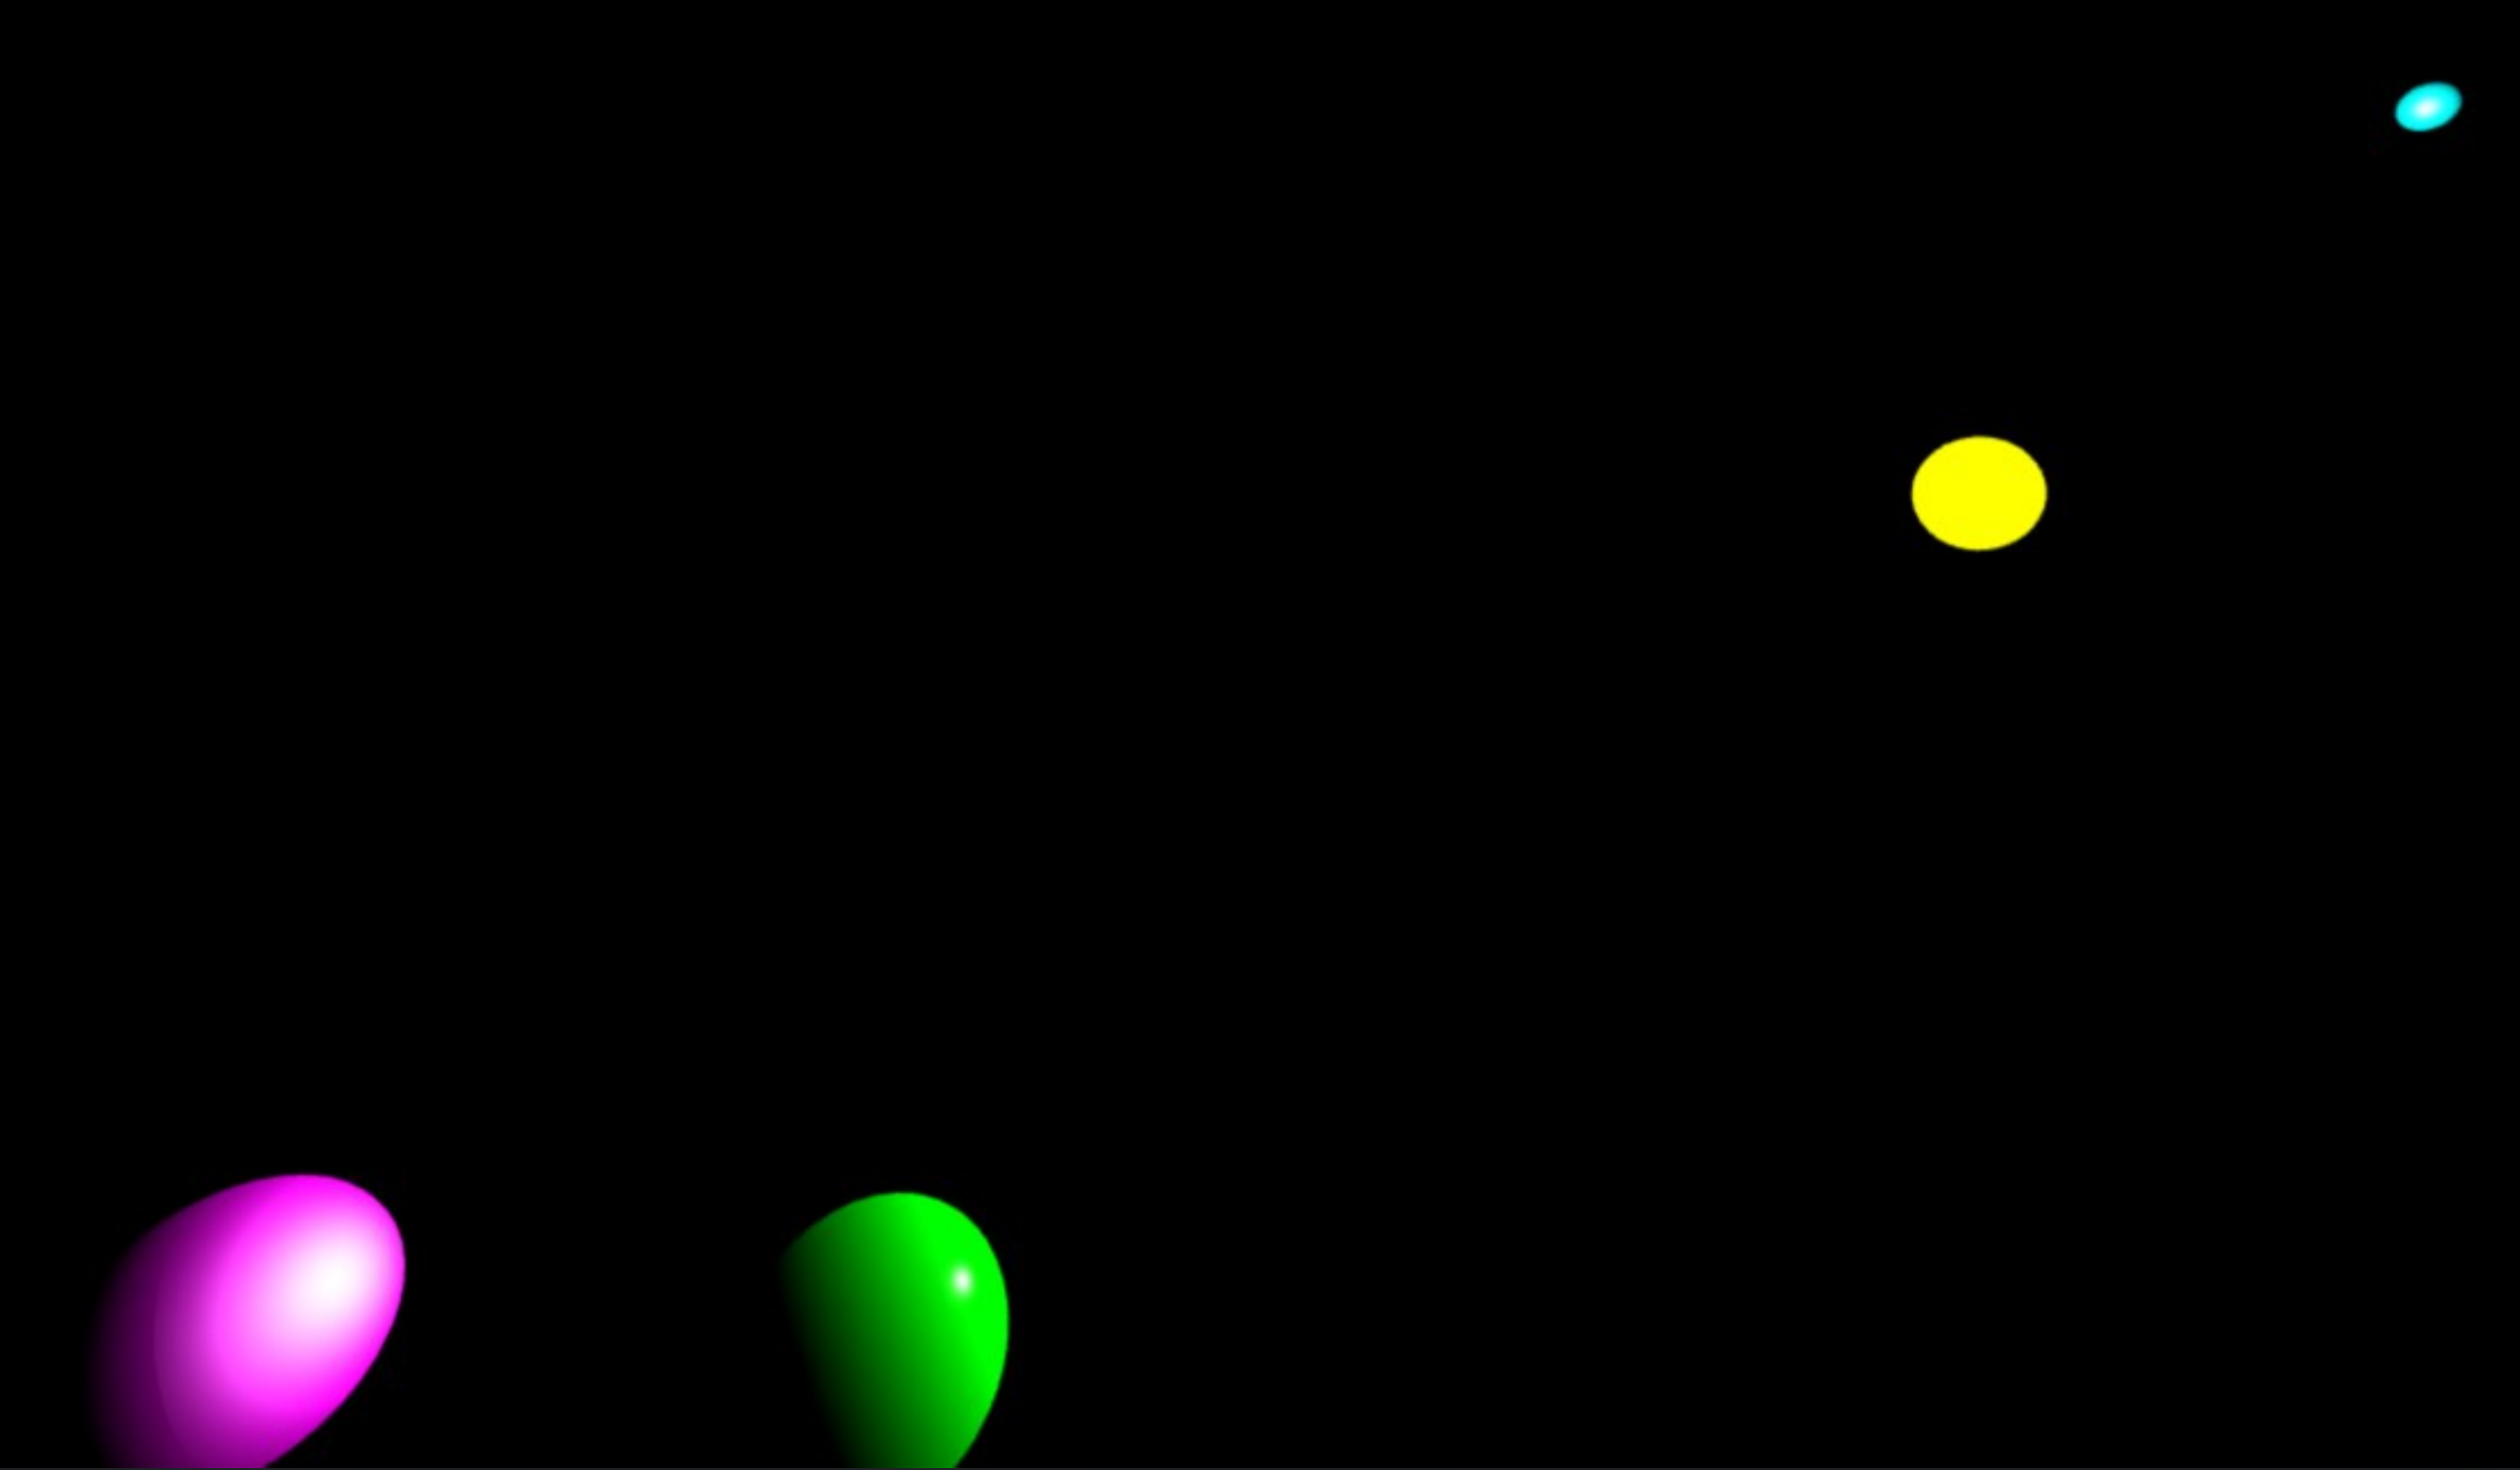
\includegraphics[width=\linewidth]{sunlight}
		\caption{Пример системы. Освещение - point-light (солнце).}
	\end{figure}
	
	
	\begin{appendices}
		\chapter{Исходный код}
		\section{index.js}
		\includelistingpretty{index.js}{JavaScript}{index.js}
		\section{WebGLCanvas.js}
		\includelistingpretty{WebGLCanvas.js}{JavaScript}{WebGLCanvas.js}
		\section{shaders.js}
		\includelistingpretty{shaders.js}{JavaScript}{shaders.js}
		\section{Camera.js}
		\includelistingpretty{Camera.js}{JavaScript}{Camera.js}
		\section{Planet.js}
		\includelistingpretty{Planet.js}{JavaScript}{Planet.js}
	\end{appendices}
	
\end{document}